\chapter{A Large Ion Collider Experiment}

\lettrine[lines=6,findent=0.pt]{A}{LICE}  (A Large Ion Collider Experiment) is a general-purpose detector at the CERN LHC~\cite{ALICE:2008ngc}. It was conceived and built to focus on the study of QCD and heavy-ion collisions. It is designed to address the physics of strongly interacting matter and the quark-gluon plasma at extreme values of energy density and temperature in nucleus-nucleus collisions. Nonetheless, its physics programme also includes proton-proton and proton-nucleus collisions, which provide reference data for the heavy-ion programme and address a number of specific strong-interaction topics for which ALICE is complementary to the other LHC detectors. During the LHC Long Shutdown 2, between 2019 and 2021, ALICE underwent a major upgrade to improve its capabilities to probe the QGP with heavy-flavour quarks, and to enable completely new measurements of the thermal emission of dielectron pairs~\cite{ALICE:2023udb}.


\section{The Large Hadron Collider}
The Large Hadron Collider (LHC) is a two-ring superconducting hadron accelerator and collider based at CERN~\cite{Evans:2008zzb}, near Geneva in Switzerland. The LHC is the world's largest circular particle accelerator with a 26.7-kilometer circumference housed in a 3.8-meter-wide tunnel buried 50 to 175 meters underground, capable of accelerating protons up to energies of $\sqrt{s} = 14$~\tev and heavy ions $({}^{208}\mathrm{Pb}^{82+})$ up to $\sqrt{s_\mathrm{NN}}~=~5.5$~\tev. 
The LHC, which was used to host the Large Electron-Positron Collider (LEP), is the final stage of a chain of accelerators that provide protons and heavy ions with sufficient energy to be injected into the LHC, illustrated in Fig.~\ref{fig:LHC}. Protons are firstly collected by stripping electrons from a gaseous hydrogen source with an electric field and then grouped into bunches. The Linear accelerator 2 (Linac~2), the first linear accelerator in the LHC injection chain, accelerates the protons to 50~\mev. The protons are then injected into the Proton Synchrotron Booster (PSB), which accelerates them to 1.4~\gev, and then into the Proton Synchrotron (PS) and the Super Proton Synchrotron (SPS), reaching 25~\gev and 450~\gev, respectively. The protons are finally injected in the LHC, where they are accelerated up to a maximum energy of 7~\tev. In the LHC, the beams are forced to follow the circular path of the ring by strong magnetic fields $(\sim 8~\mathrm{T})$ produced by superconducting dipole magnets. Other magnets are used to steer and focus the beams in the interaction points. 

\begin{figure}[htb]
    \centering
    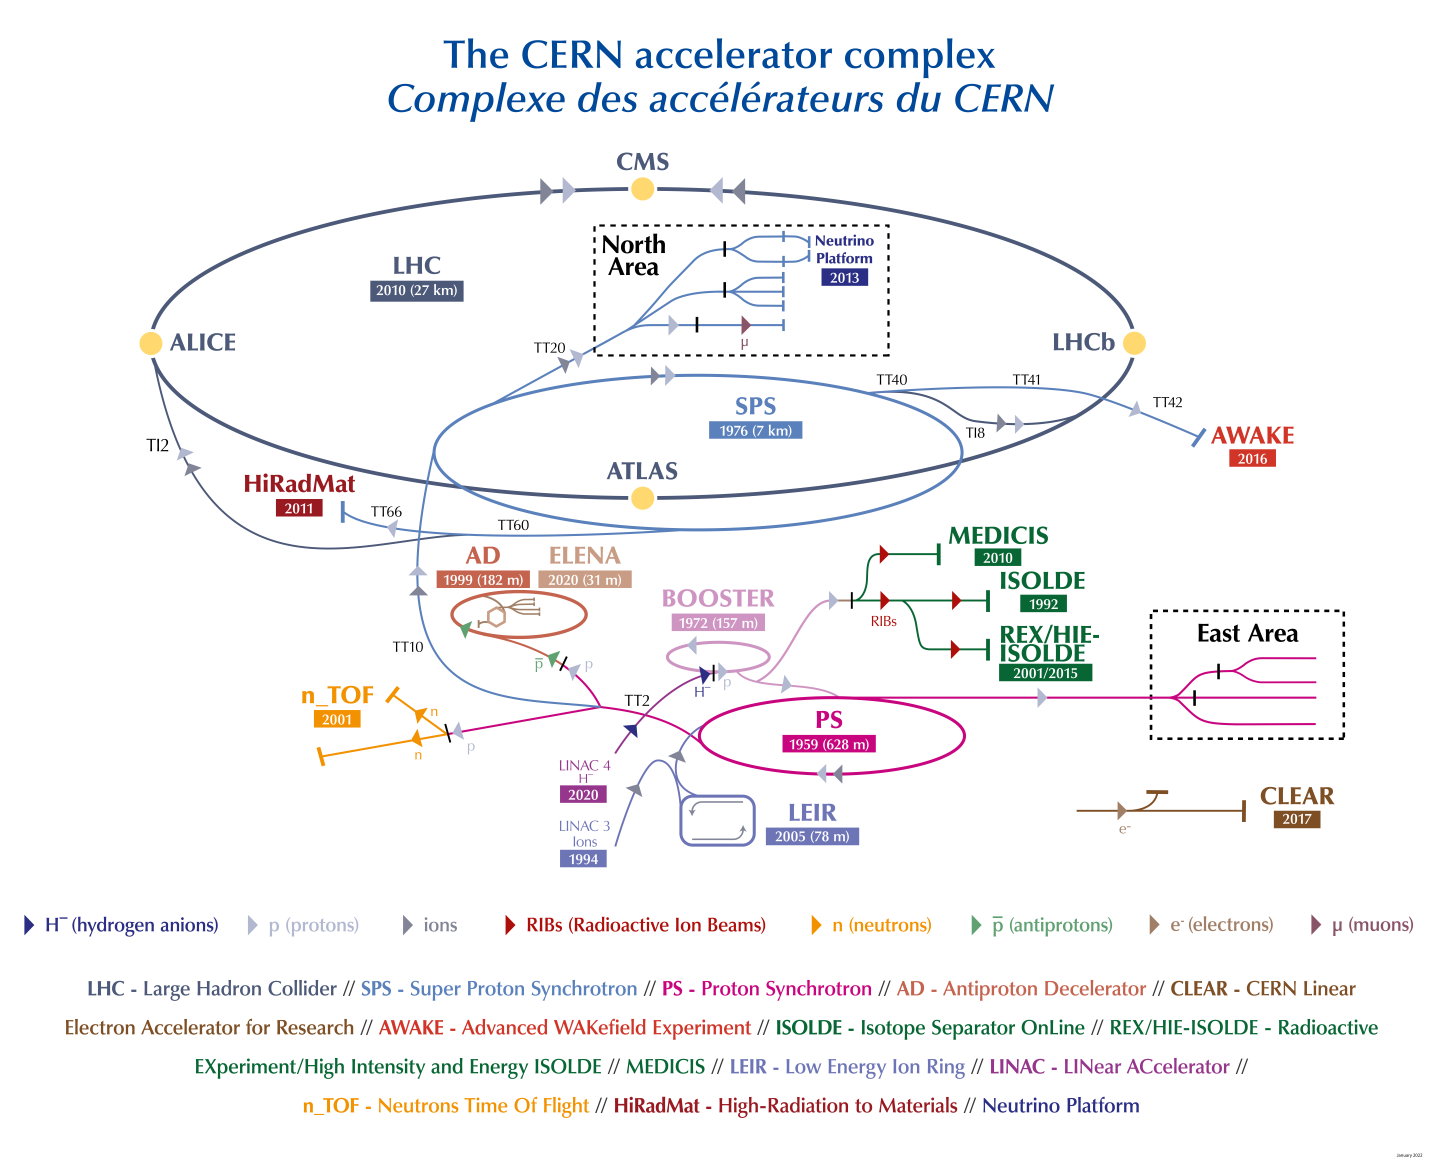
\includegraphics[width=\textwidth]{Figures/Chapter 3/LHC_Scheme.png}
    \caption{The Large Hadron Collider (LHC) accelerator complex at CERN.}
    \label{fig:LHC}
\end{figure}

Heavy-ion acceleration follows a similar path. The Pb ions (Pb$^{25+}$ -- Pb$^{28+}$) are extracted in the Electron-Cyclotron Resonance (ECR), and are focused in a Radio-Frequency Quadrupole (RFQ) using only electric fields. Pb$^{28+}$ ions with momentum of 2.5~\kevc are selected with a spectrometer, and are accelerated to 4.2~\mevc in the Linear accelerator 3 (Linac~3). A first \SI{0.5}{\micro\meter} copper stripping foil is then used to increase the charge state of the ions to Pb$^{53+}$. The PSB and PS accelerate the ions to 95.4~\mev A and 5.09~\gev. After the PS, a copper stripper ($\sim 1~\mathrm{mm}$) is used to further ionise the Pb ions to Pb$^{82+}$, which are then accelerated to 158~\gev in the SPS. The ions are finally injected into the LHC, where they are accelerated to 2.76~\tev per nucleon.

The LHC can collide protons with protons, protons with heavy ions, and heavy ions with heavy ions. The LHC has four main interaction points, where the four main detectors are located: A Large Ion Collider Experiment (ALICE), A Toroidal LHC ApparatuS (ATLAS), Compact Muon Solenoid (CMS), and LHC-beauty (LHCb). The four experiments were conceived and built to address different physics topics: ATLAS and CMS are general-purpose detectors designed to study the Higgs boson, which they discovered in 2012~\cite{ATLAS:2012yve,CMS:2012qbp} and to search for physics beyond the Standard Model; LHCb is dedicated to the measurement of beauty quarks as proxy for CP violation studies, and to the study of matter-antimatter asymmetry. ALICE is the only detector at the LHC that is dedicated to the study of QCD rather than the electroweak sector of the Standard Model. A more detailed description of the ALICE detector is given in the following sections.

\textcolor{red}{aggiungere luminosità istantanea}

\section{The ALICE experiment}
The physics programme of ALICE revolves around the study of the properties of strongly interacting matter at the extreme values of energy density and temperature reached in ultra-relativistic heavy-ion collisions. This unique environment poses several challenges, the most stringent one being the need to carry out measurements in a very high multiplicity environment. Originally, estimates for the charged particle multiplicity density at mid-rapidity in central Pb--Pb collisions ranged from $\de N/\de\eta = 2000$ up to almost $\de N/\de\eta = 8000$. Detectors with high granularity, fast readout capabilities, and highly radiation hardness were thus needed. The ALICE detector was designed to meet these requirements, and to provide a comprehensive set of measurements to study the properties of the QGP. The ALICE apparatus is shown in Fig.~\ref{fig:ALICE}. It is based on a central barrel, covering full azimuth ($0 < \varphi < 2\pi$) and the pseudorapidity region $\lvert \eta\rvert <0.9$ and a forward muon system with a dipole magnet providing a total bending power of 3~Tm, covering full azimuth and the pseudorapidity interval $-4.0 < \eta < -2.5$.

\begin{figure}
    \centering
    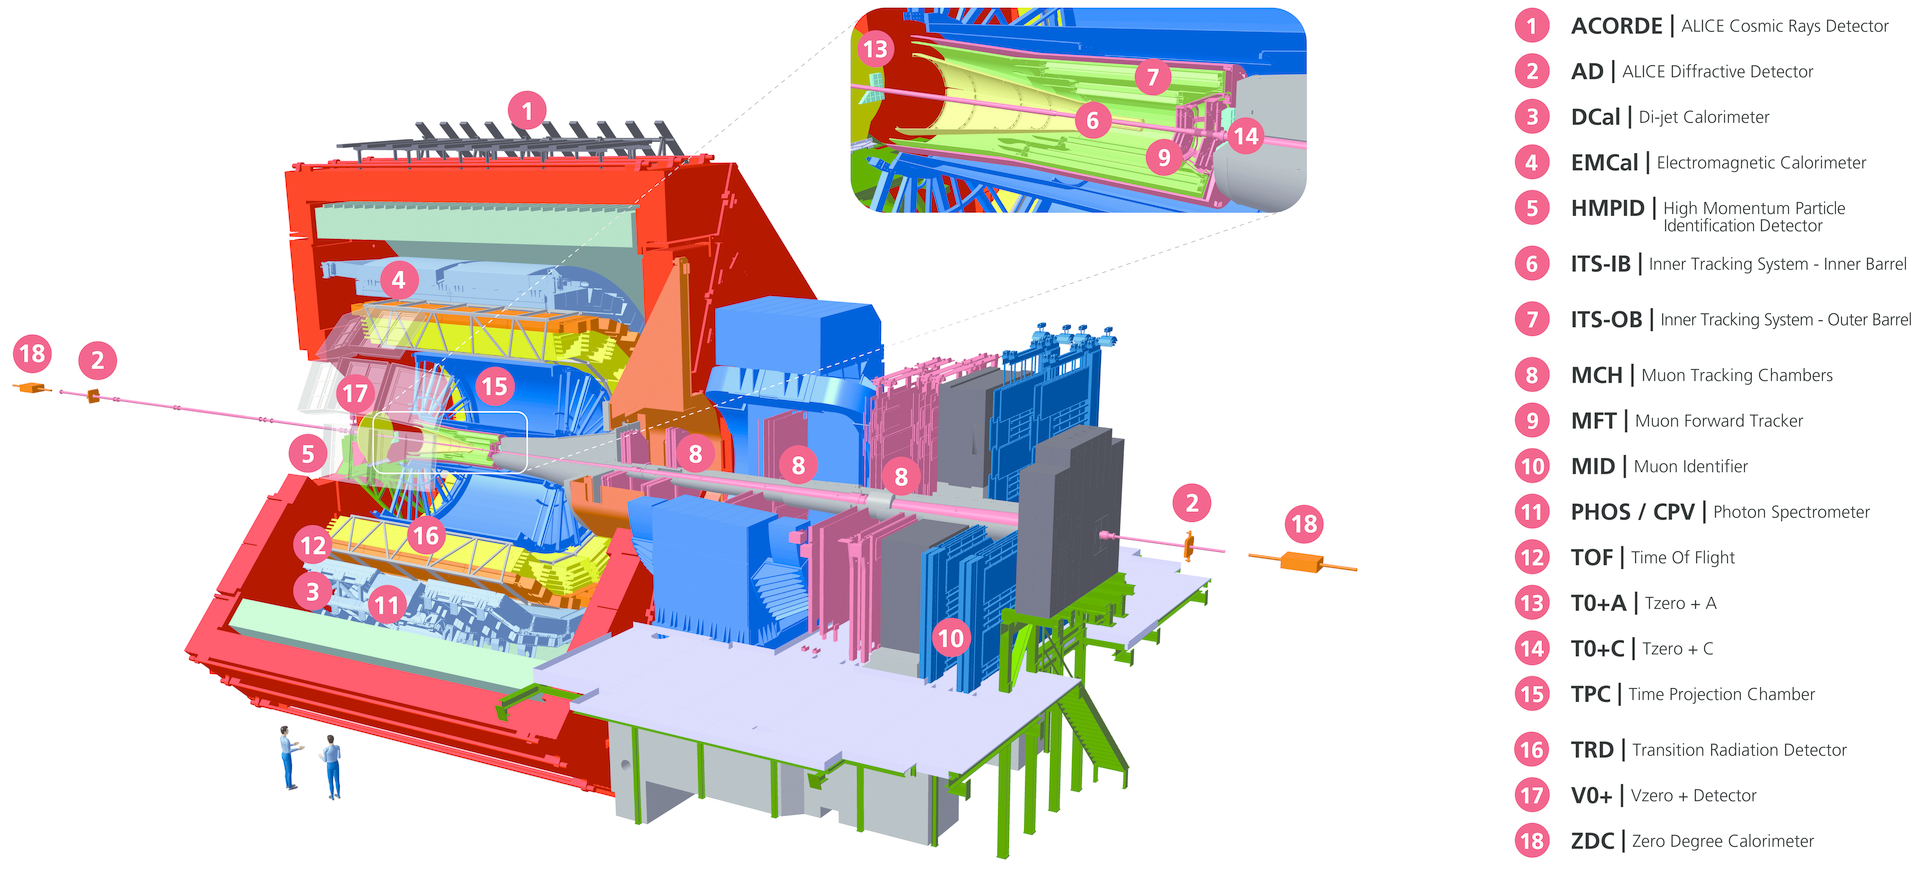
\includegraphics[width=\textwidth]{Figures/Chapter 3/ALICE_Scheme.png}
    \caption{The ALICE experimental apparatus. The top right panel shows a zoom of the ITS, T0-A, T0-C and MFT detectors. Figure from ALICE figure repository~\cite{ALICE_figures}.}
    \label{fig:ALICE}
\end{figure}

The ALICE coordinate system is a right-handed system with the $z$-axis pointing along the beam direction, in the direction away from the muon arm, the $y$-axis pointing vertically up, and the $x$-axis pointing horizontally towards the center of the LHC. The nominal interaction point is the origin of the coordinate system. The two sides of the detector along the beam axis are referred to as the C-side, where the muon arm is positioned, and the A-side, where the FV0 is positioned. The polar angle $\theta$ is defined with respect to the $z$-direction and $\varphi$, the azimuthal angle, increases counter-clockwise
starting from the $x$-axis towards the CMS side.


The central barrel is enclosed in the L3 solenoid, which has an internal length of 12.1~m and a radius of 5.75~m, providing a magnetic field of 0.5~T. The L3 experiment was a detector at the Large Electron-Positron Collider (LEP) at CERN~\cite{Myers:1991ym}, which operated from 1989 to 2000, and was built in the cavern where ALICE is now located. The central barrel detector system is designed for efficient tracking in the high track-density environment of heavy-ion collisions, covering transverse momenta from $\sim100~\mevc$ to $\sim100~\gevc$ with excellent hadron and electron identification capabilities. It is also capable of the reconstruction of primary and secondary vertices with a resolution $\sim\SI{40}{\micro\meter}$. This allows for precise measurements of heavy-flavour hadrons, which typically decay at a distance of $\sim\SI{100}{\micro\meter}$ from the primary vertex. The L3 magnet hosts the Inner Tracking System (ITS), the Time Projection Chamber (TPC), the Transition Radiation Detector (TRD), the Time-Of-Flight (TOF) detector, the High-Momentum Particle Identification Detector (HMPID), and the Electromagnetic Calorimeter (EMCal). The central barrel also includes forward detectors such as the Muon Forward Tracker (MFT) and the Fast Interaction Trigger (FIT). The muon detectors cover the forward pseudorapidity range $-4.0 < \eta < -2.5$ and are made of absorbers, a large dipole magnet, planes of triggering Resistive Plate Chambers (RPC) and tracking multiwire proportional chambers (MWPC).

In the following sections, the main components of the ALICE detector are described in detail, following the path of a particle produced at mid-rapidity. The upgrades of the ALICE detectors during the LHC Long Shutdown 2 will be highlighted.

\subsection{ALICE upgrades overview}
The ALICE detector underwent a major upgrade during the LHC Long Shutdown~2, between 2019 and 2021, which renewed the experiment, now referred to as ALICE~2. The upgrade aimed at significantly improving the capabilities of ALICE to probe the QGP with heavy-flavour quarks, and enabling completely new measurements of the thermal emission of dielectron pairs. To achieve these goals, the ALICE detector was improved by enhancing the tracking capabilities of the central barrel detectors and increasing the readout rate of the detectors to expand the collected data sample. The Inner Tracking System (ITS) was replaced with a new detector, the ITS-2, a thinner and lighter detector with the first layer closer to the interaction point, which improves the pointing resolution by a factor of 3 in the transverse direction and a factor 6 in the longitudinal direction, as shown in Fig~\ref{fig:ITS_res}.

\begin{figure}[htb]
    \centering
    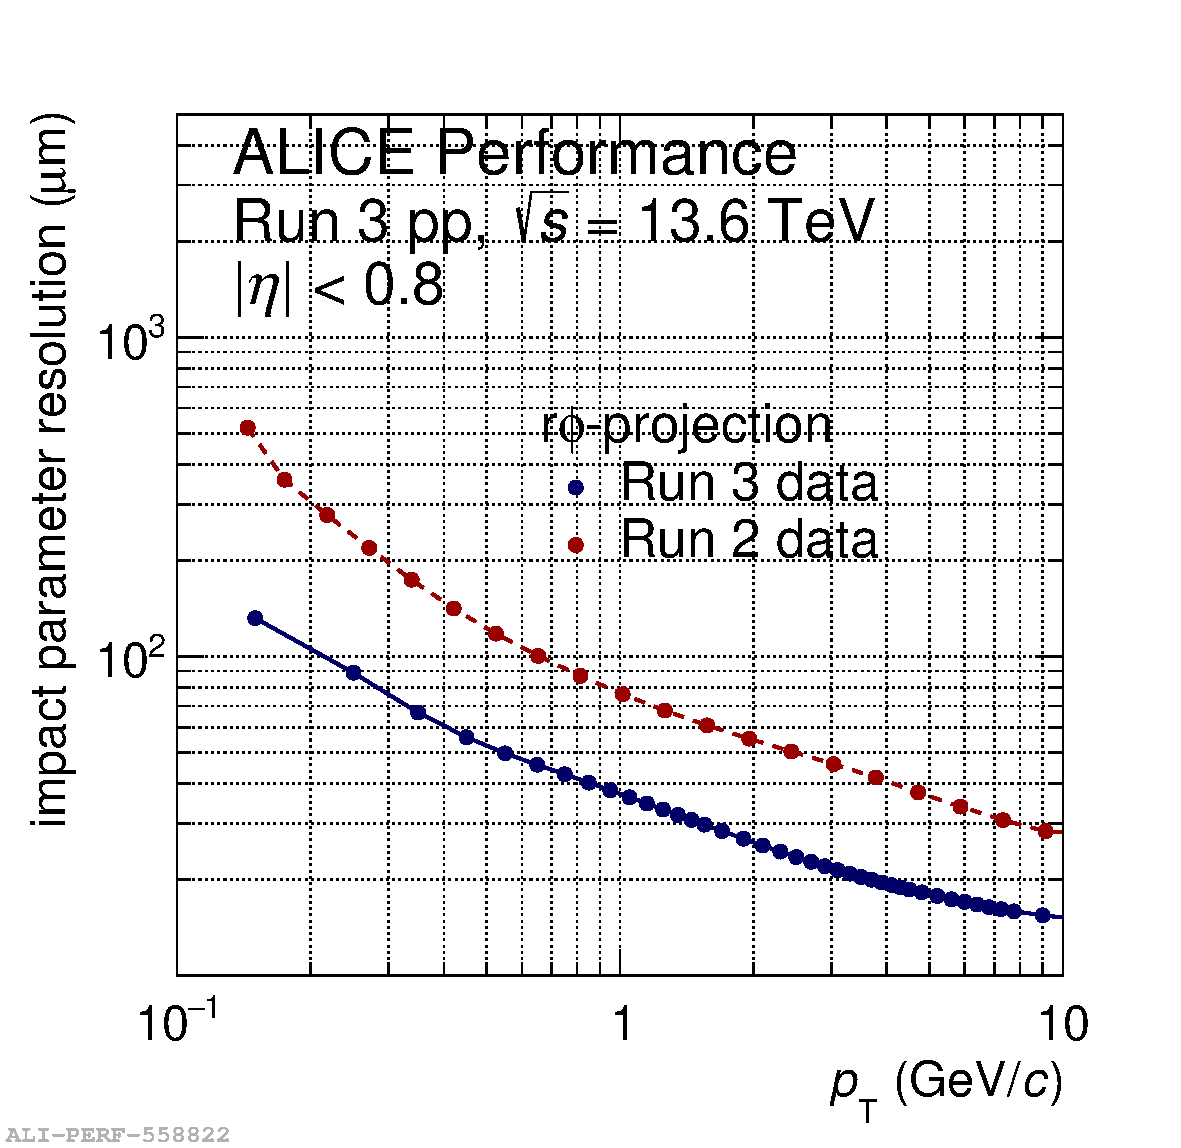
\includegraphics[width=0.7\textwidth]{Figures/Chapter 3/sigmadcaxy_run2vsrun3data_qm.pdf}
    \caption{Impact parameter resolution in $r\phi$ as a function of \pt in pp collisions at \thirteen from Run 3 data compared with the same quantity measured in collisions at $\sqrt{s} = 13$~\tev from Run 2 data. Figure taken from ALICE figure repository~\cite{ALICE_figures}.}
    \label{fig:ITS_res}
\end{figure}

The upgrade strategy for the enhanced readout rate is based on the LHC plans to increase the luminosity of Pb--Pb collisions progressively after the LHC Long Shutdown 2, eventually reaching an interaction rate of about 50~kHz (from less than 1~kHz during LHC Run~1 and 2 data-taking periods), i.e. instantaneous luminosity of $\mathcal{L} = 6\times10^{27}~\mathrm{cm}^{-2}~\mathrm{s}^{-1}$. At these high interaction rates, each TPC drift time period of $\sim\SI{100}{\micro\second}$ will contain on average 5 Pb--Pb events. It was therefore decided to use a continuous, untriggered readout strategy. With the MWPC used in ALICE~1 for the TPC readout, the ion backflow into the drift region had to be suppressed by active gating, limiting the readout rate to about 700 Hz for Pb--Pb collisions. This is overcome in ALICE~2 by using a readout based on Gas Electron Multiplier (GEM) foils, which reduce the ion backflow and resulting space charge in the TPC to a level that can be corrected for while operating the detector with Pb--Pb interaction rates up to 50 kHz. 

To synchronise the continuous data stream across all readout and processing branches, the data stream is divided into time frames (TF) of nominal length of 128 LHC orbits ($\sim11$~ms). Each TF is subdivided into heartbeat frames (HBF) with a length corresponding to an orbit of $\sim\SI{89.4}{\micro\second}$. The detector data are time stamped with a precision of an LHC bunch crossing of 25~ns. 

The Online-Offline (\osq) software framework has been developed to allow for distributed and efficient processing of this unprecedented amount of data. Because of the continuous readout in Run~3, the vertex-to-track association is no longer unambiguous. Therefore, in place of the analysis data model used in Runs~1 and 2, based on the hierarchical structure of the "event content", the analysis data model for Run~3 is based on a columnar data format, where collisions and tracks are represented as separate tables, connected by an index. This maps naturally on a "flattened" structure-of-arrays data format. Hence, the columnar data format provided by Apache Arrow~\cite{ApacheArrow} was chosen. The new framework ensures a unified and coherent computing environment from data taking up to analysis. Throughout all stages of the data processing, the timeframe represents the minimal processing unit. 

The result of asynchronous reconstruction is the Analysis Object Data (AOD) format, with the best calibration available. During processing the content of an AOD timeframe is kept contiguously in shared memory allowing efficient application of parallel execution and pipelining. AODs are stored as ROOT trees, exploiting their columnar storage format. The ROOT trees are then used to perform physics analyses. 

\subsection{Inner Tracking System}
The Inner Tracking System (ITS) is the innermost detector of the ALICE apparatus, and is designed to provide precise tracking and vertexing capabilities in the high-multiplicity environment of heavy-ion collisions. The ITS upgrade is one of the key improvements of the ALICE~2 detector. The ITS~1 was a six-layer silicon detector, with two layers of Silicon Pixel Detectors (SPD), two layers of Silicon Drift Detectors (SDD), and two layers of Silicon Strip Detectors (SSD). The ITS~1 was replaced by the ITS~2, which brought a plethora of improvements: i. a new beryllium beam pipe with an outer radius reduced from 28~mm to 18~mm allows for an innermost detector layer closer to the interaction point, from 39~mm to 22.4~mm; ii. an increased granularity for all layers, which are now silicon pixel detectors with a cell size of $\SI{29.24}{\micro\meter}\times\SI{26.88}{\micro\meter}$; iii. the number of layers for the inner barrel was increased from two to three, raising the total number of layers from six to seven; iv. the material budget was reduced to $0.36\%~X_0$ ($1.10\%~X_0$) per layer for the innermost (outer) layers. A schematic view of the ITS~2 is presented in Fig.~\ref{fig:ITS}, while the main layout parameters are summarised in Table~\ref{tab:ITS2_params}.

\begin{figure}
    \centering
    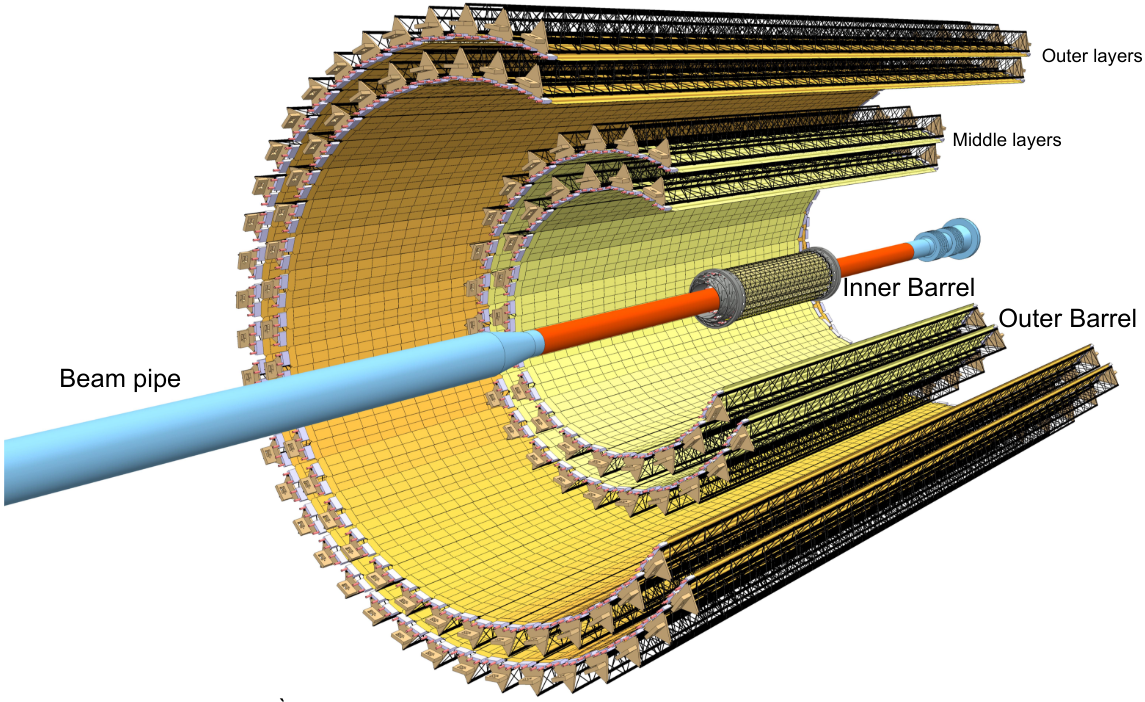
\includegraphics[width=0.7\textwidth]{Figures/Chapter 3/ITS_Scheme.png}
    \caption{Schematic view of the ALICE ITS-2. Figure taken from Ref.~\cite{ALICE:2023udb}.}
    \label{fig:ITS}
\end{figure}

\begin{table}[t]
    \centering
    \caption{Main layout parameters of the new ITS2. Taken from Ref.~\cite{ALICE:2023udb}.}
    \begin{tabular}{c|ccccc}
    \toprule
    Layer no. &	Average&	Stave&	No. of &No. of &Total no.\\
    &	radius&length&staves&HICs/	&of chips\\
    &	(mm)&(mm)& &stave	&\\
    
    \midrule
    0	&23 & 271 & 12 & 1&108\\
    1	&31 & 271 & 16	& 1&144\\
    2	&39 & 271 & 20	& 1&180\\
    3	&196 & 844 & 24 & 8	&2688\\
    4	&245 & 844 & 30 & 8	& 3360\\
    5	&344 & 1478	&42 & 14 &	8232\\
    6	&393 & 1478	& 48 & 14 &	9408\\
    
    \bottomrule
    \end{tabular}
    \label{tab:ITS2_params}
\end{table}

In addition, the ITS~2 uses ALPIDE~\cite{AglieriRinella:2017lym} chips, i.e., Monolithic Active Pixel Sensors~\cite{Snoeys:2014daa} (MAPS) implemented in a 180~nm CMOS technology for imaging sensors provided by TowerJazz~\cite{Senyukov:2013se}.

MAPS are an evolution of the hybrid pixel sensors which have been widely used in the past by several experiments~\cite{ALICE:2008ngc,CMS:1997tlf,Aad:2008zz,Bediaga:2013tje}. Hybrid pixel sensors are made of an active layer, typically made of silicon, and a readout layer, connected to the active layer by bump-bonding. On top of being expensive and complex, the bump-bonding operation introduces additional material in the detector, which increases the material budget of the detector. MAPS, on the other hand, are monolithic sensors, where the active layer and the readout layer are integrated into the same silicon wafer. This significantly reduces the material budget of the detector. The ALPIDE chip is a 15~mm$\times$30~mm chip, with a pixel size of $\SI{29.24}{\micro\meter}\times\SI{26.88}{\micro\meter}$, and a total of 512$\times$1024 pixels. Each pixel cell contains a sensing diode, a front-end amplifier and a shaping stage, a discriminator, and a digital section. The digital section includes a multi-event buffer with three hit storage registers and a pixel mask register. At the time of writing this Thesis, the ITS~2 is the largest-scale application of MAPS in a high-energy physics experiment.

\subsection{Time Projection Chamber}
\begin{figure}
    \centering
    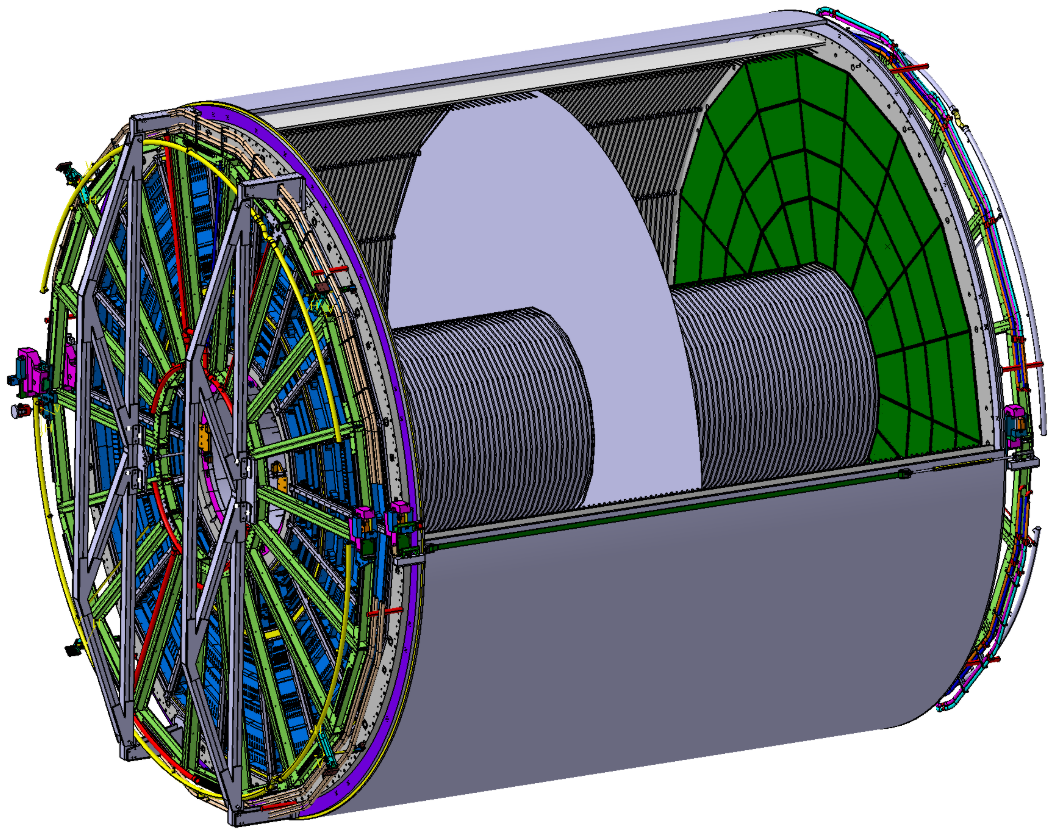
\includegraphics[width=0.7\textwidth]{Figures/Chapter 3/TPC_Scheme.png}
    \caption{Schematic view of the ALICE TPC. Figure taken from Ref.~\cite{ALICE:2023udb}.}
    \label{fig:TPC}
\end{figure}
The Time Projection Chamber is the main tracking detector of the ALICE experiment, and is designed to provide precise \pt measurements and particle identification via $\de E/\de x$ of charged particles. The TPC is a large cylindrical detector with a length and outer diameter of about 5 m, resulting in a volume of 88~m$^3$ filled with a gas mixture of Ne-CO$_2$-N$_2$ (90-10-5). It covers a symmetric pseudorapidity interval around midrapidity ($\lvert\eta\rvert < 0.9$) at full azimuth. The field cage has a high-voltage (100~kV) electrode in its center, which divides the active volume into two halves. The inner diameter of the central field cage drum is 114~cm, providing the necessary space for the installation of the ITS.  Each of the two endplates houses 18 inner and outer readout chambers (IROCs and OROCs), which are arranged in pairs to form 18 equal azimuthal sectors.

During Runs~1 and 2, the readout chambers were based on MWPCs, which have to be operated with an active ion gating grid in order to prevent the ions produced in the amplification region from reaching the active drift volume, which could lead to space-charge distortions. The ambitious physics program of the ALICE experiment requires the elimination of the intrinsic trigger rate limitation to about 3 kHz of the original MWPC-based TPC, imposed by the operation of the active ion gating grid.

Operating the TPC at a collision rate of 50 kHz implies that on average five collision events pile up within the TPC readout time window of about $\sim\SI{100}{\micro\second}$. This excludes triggered operation and defines the need for continuous readout, requiring the exploitation of gas amplification techniques capable of providing sufficient ion blocking without an active gate. At the same time, the readout system must ensure that the $\de E/\de x$ resolution of the TPC is preserved.

GEMs~\cite{Sauli:1997qp} represent a valid solution to overcome the limitations of MWPCs. Sufficient ion blocking can be achieved by stacking four GEMs using standard (S, \SI{140}{\micro\meter}) and large (LP, \SI{250}{\micro\meter}) hole pitch in an S-LP-LP-S configuration and by adjusting the gain share among the four layers. The latter optimisation allows for efficiently blocking the ions, most of which are produced in the last amplification step, i.e. the closest to the readout pad. A careful choice of hole patterns is made to avoid the accidental alignment of holes in subsequent layers. 

Thanks to this design, the detector is capable of satisfying the requirements for Run~3 operation, with an ion backflow below 2\% and a local energy resolution at the $^{55}$Fe-peak below 14\%.

\subsection{Time-of-Flight}
The TOF detector is a large area detector covering the central pseudo-rapidity region ($\lvert\eta\rvert < 0.9$), extending from an inner radius of 370~cm to an external one of 399~cm. Its main purpose is the particle identification in the intermediate momentum range, achieving a $\pi$/K and K/p separation better than 3 times the time-of-flight resolution below about 2.5~\gevc for pions, and up to 4~\gevc for protons. The TOF detector is built with a modular structure corresponding to 18 sectors in $\varphi$ and five modules along the beam direction. It is based on Multi-gap Resistive Plate Chambers (MRPCs)~\cite{Wang:2020iwn}, which are capable of providing a time resolution of about 40~ps~\cite{ALICE:2008ngc}. The gas mixture used in the MRPCs is $\mathrm{C_2H_2F_4 (90\%), i\text{-}C_4H_{10} (10\%), SF_6 (5\%)}$, which proved to be a good solution as no significant ageing effects were observed after 3.5 times the dose foreseen in the first 10 years of operation.

Together with the ITS and TPC, the TOF is the detector in charge of providing event-by-event identification of large samples of pions, kaons, and protons. The mass of a given particle is estimated from the measurement of its time-of-flight:
\begin{equation}
    m = p \cdot \sqrt{\left(\frac{t_\mathrm{flight}}{L}\right)^2 - 1}\quad ,
\end{equation} 
where $p$ is the particle's momentum, measured from the curvature of its trajectory, $t_\mathrm{flight}$ is the time-of-flight, and $L$ is the track length. \textcolor{red}{si trascura la curvatura?} The time-of-flight is evaluated as the difference between the time of arrival of the particle at the TOF $t_\mathrm{hit}$ and the time of the collision $t_0$, estimated using a timing signal from the FT0 detector, which is described in Sec.~\ref{subsec:FIT}: $t_\mathrm{flight} = t_\mathrm{hit} - t_0$.

\subsection{Fast Interaction Trigger}\label{subsec:FIT}
The Fast Interaction Trigger (FIT) serves as the main forward trigger, luminometer, and interaction-time detector. It also provides an initial indication of the vertex position and determines the multiplicity, centrality, and reaction plane of heavy-ion collisions. The FIT consists of five distinct detector stations, positioned at different locations along the beam line: the FT0 (-A and -C), the FV0, and the FDD (-A and -C). An illustration of the FIT is shown in Fig.~\ref{fig:FIT}.

\begin{figure}[htb]
    \centering
    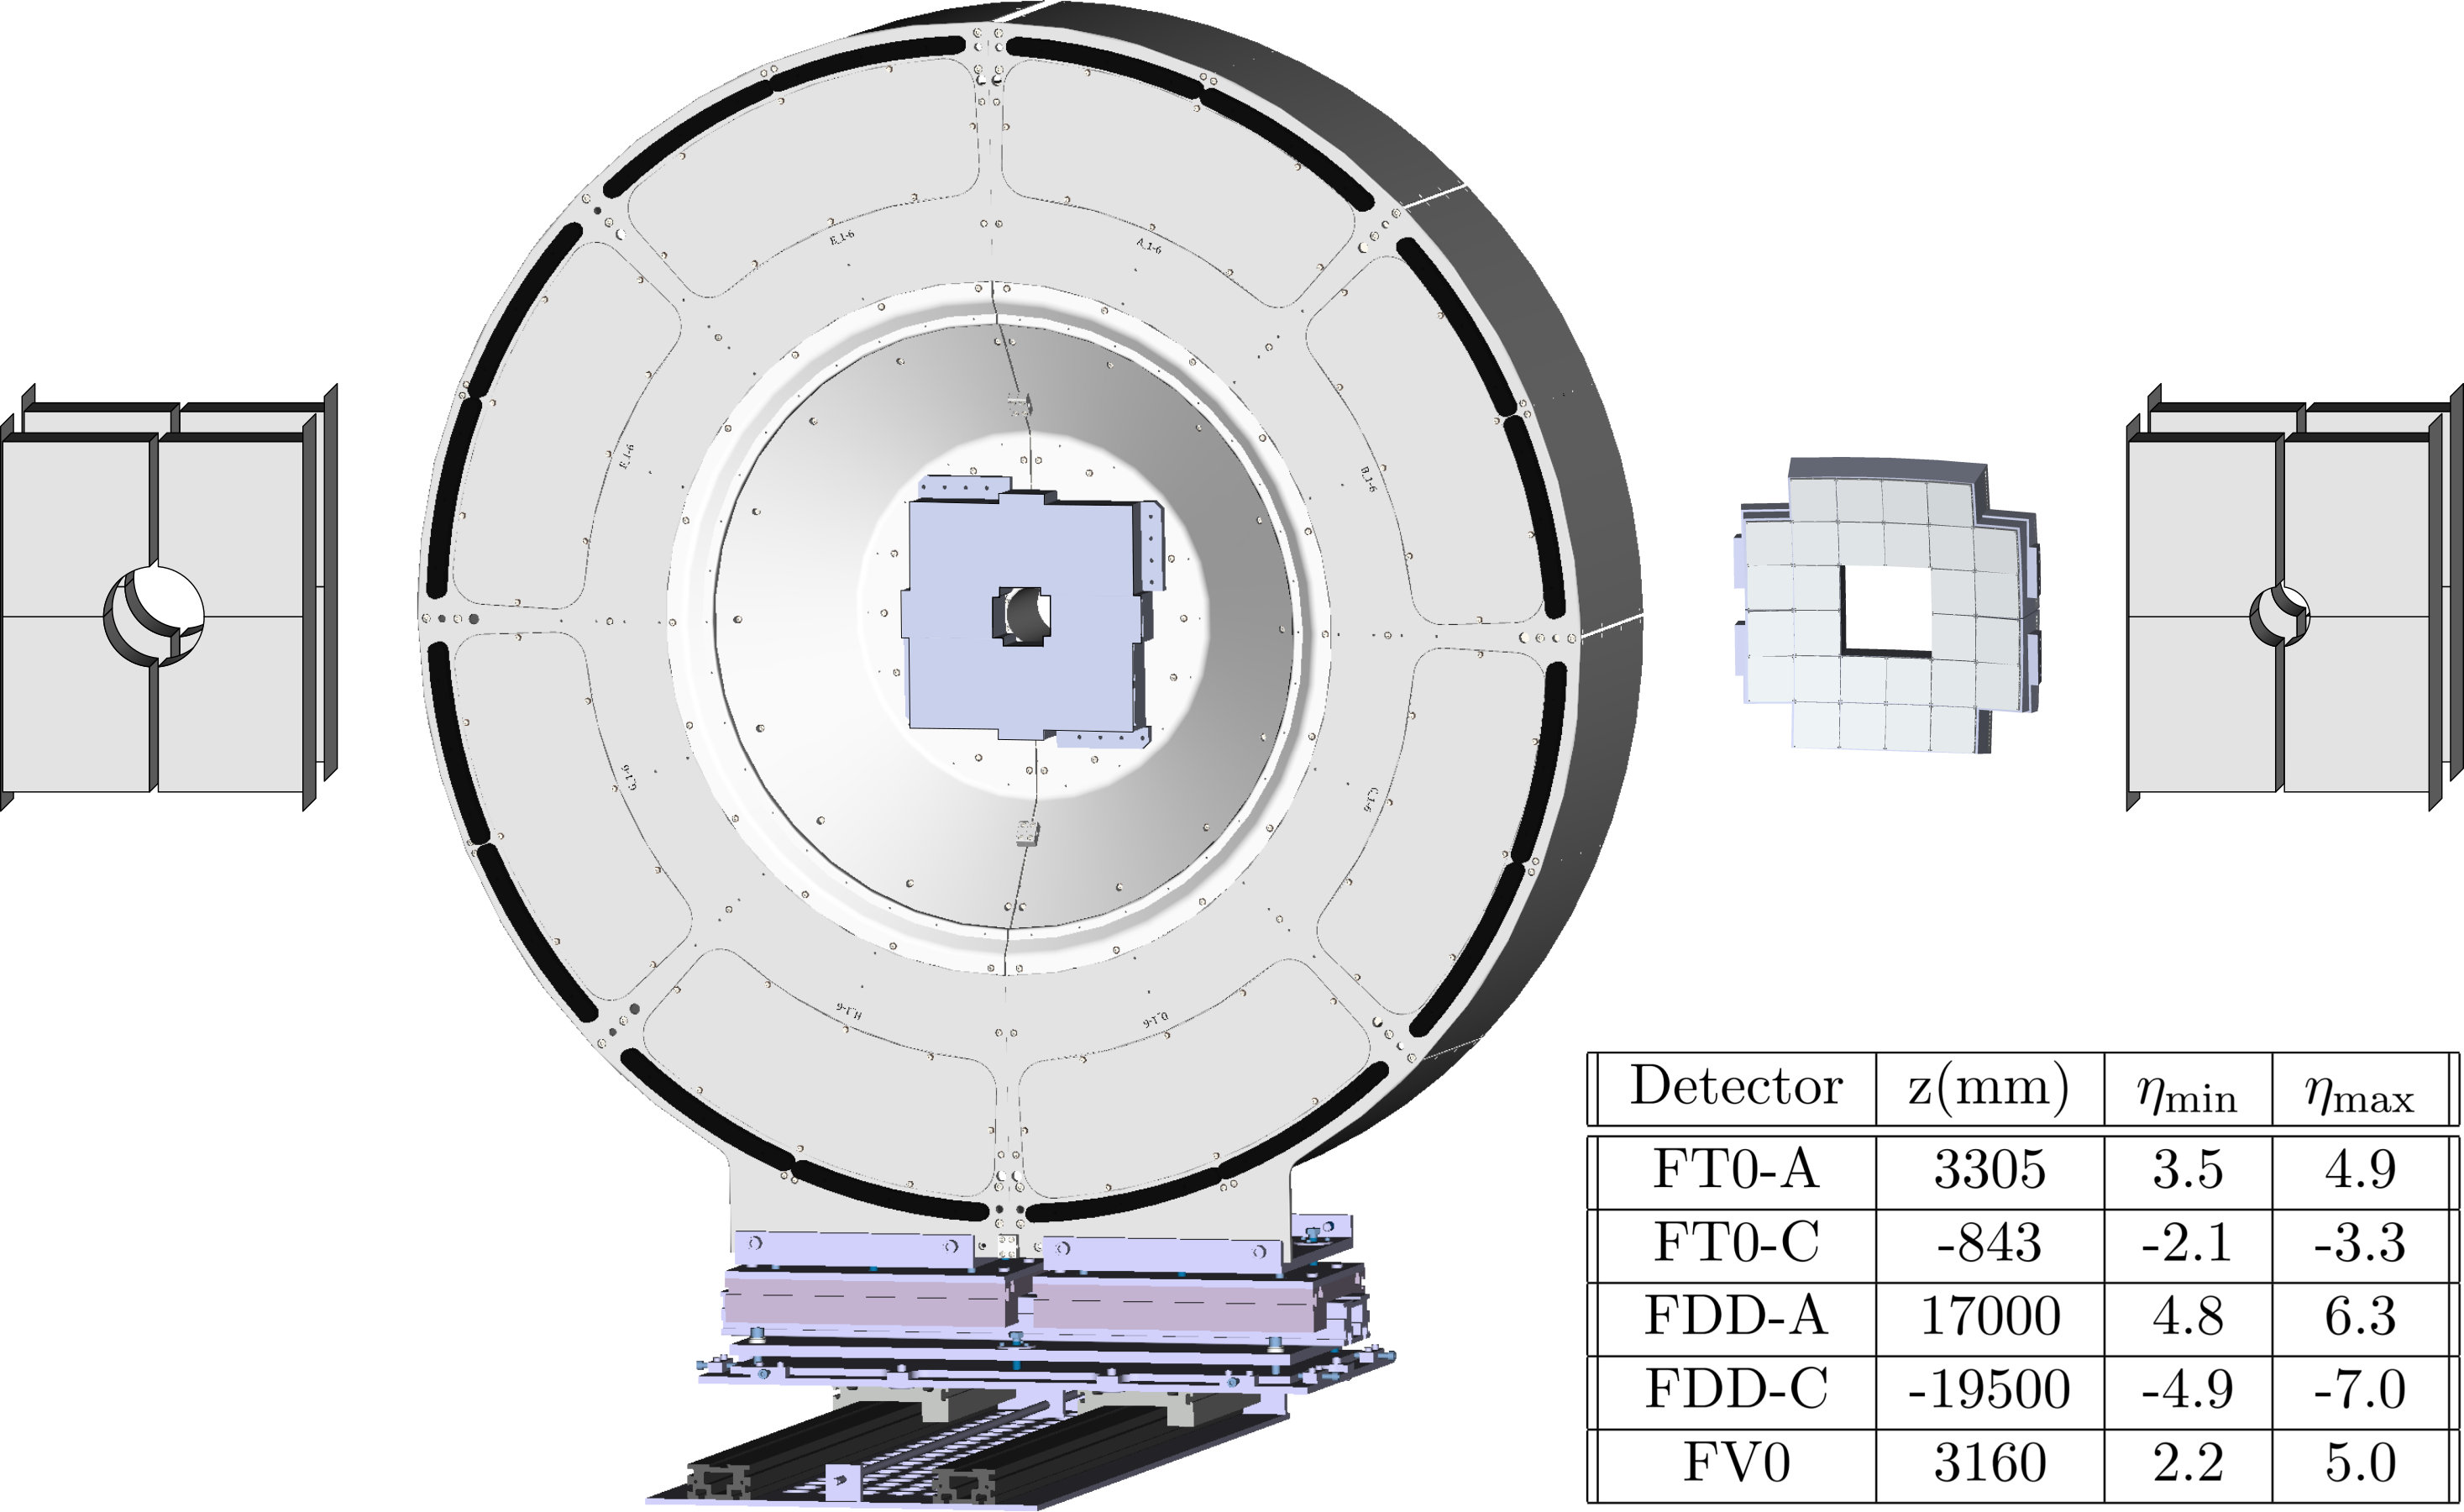
\includegraphics[width=0.7\textwidth]{Figures/Chapter 3/FIT_Scheme.png}
    \caption{View of the FIT detectors illustrating the relative sizes of each component. From left to right, the FDD-A, FT0-A, FV0, FT0-C, and FDD-C are shown. The FT0-A and FV0 systems have a common mechanical support: the former is the small quadrangular structure in the centre of the large, circular FV0 support. The inset table lists the distance from the interaction point and the pseudorapidity coverage for each component. Figure taken from Ref.~\cite{ALICE:2023udb}.}
    \label{fig:FIT}
\end{figure}

\subsubsection{FT0}

The FT0 is made of two arrays of quartz Cherenkov radiators, FT0-A and FT0-C, coupled to MicroChannel Plate-based photomultipliers (MCP). Its main task is to determine the vertex position with an accuracy of a few centimeters, and to provide the interaction time with the precision needed by the TOF system for event-by-event particle identification. An optimal time resolution ($<50$~ps) is therefore required. The FT0-A is located at 3.3~m from the nominal interaction point, while the FT0-C is only 84~cm from the interaction point. To provide a reliable indication of the time of a collision, the FT0-C support has a convex shape, to ensure that each of the 112 quartz radiators is positioned at a distance of 84 cm from the nominal interaction point. On the contrary, the FT0-A is characterised by a planar geometry, made of 96 quartz radiators. To achieve the best possible timing resolution, the signal path from each MCP anode to the front-end electronics has the same length. The intrinsic time resolution of each quadrant is $\sigma_t \sim 13$~ps

\subsubsection{FV0}
The FV0 is a large, segmented scintillator disk. It achieves a single MIP time resolution of about 200~ps with a very uniform response across the entire detection surface thanks to its light collection scheme, shown in Fig.~\ref{fig:FV0}. The active element of FV0 is a 4~cm-thick plastic scintillator divided into five concentric rings of equal pseudorapidity coverage. The outer diameter of the largest ring is 144~cm and the inner diameter of the smallest is 8~cm. The four inner rings are subdivided into eight sectors of 45 degrees each, while the outermost ring, due to its large area, has 16 sectors. A grid of equal-length fibers is attached to the back side of the scintillator, where they are attached to the photomultiplier tubes (PMTs). Each sector is read out by an independent PMT to provide a minimum bias and multiplicity trigger, when coupled to the FT0 information.

\begin{figure}[htb]
    \centering
    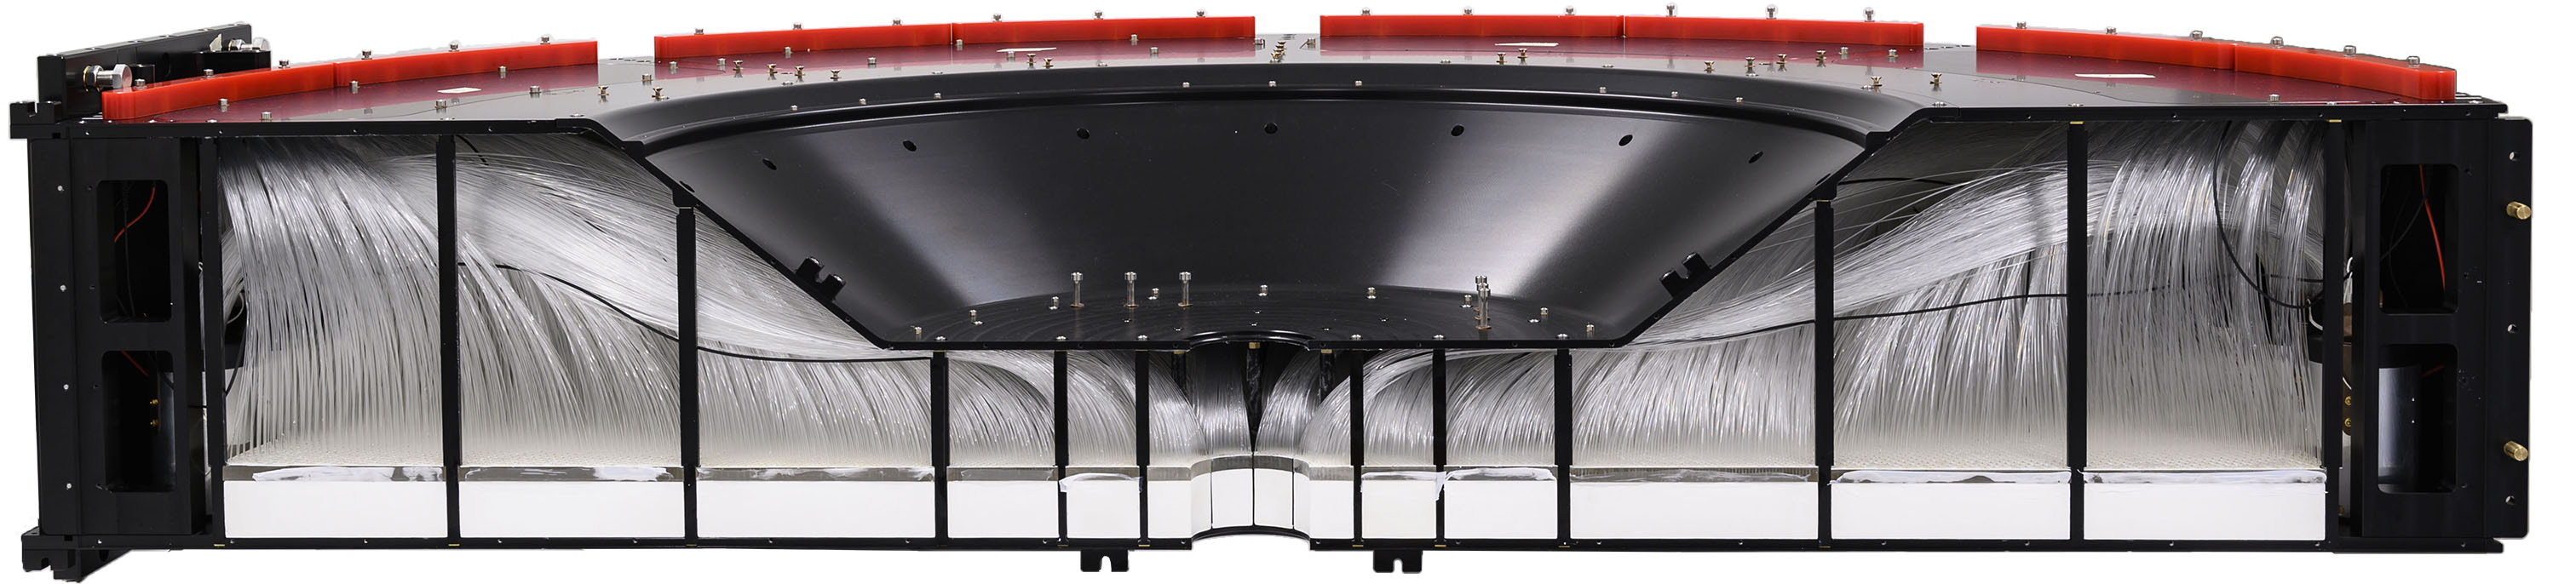
\includegraphics[width=0.7\textwidth]{Figures/Chapter 3/FV0_Scheme.jpg}
    \caption{Photograph of one half of the FV0 detector. Figure taken from Ref.~\cite{ALICE:2023udb}.}
    \label{fig:FV0}
\end{figure}

\subsubsection{FDD}
The FDD is made of two similar arrays, FDD-A and FDD-C, surrounding the beam pipe on opposite sides of the nominal interaction point, and consisting of eight rectangular scintillator pads each, arranged into two overlapping layers of four sectors. A quadrant was removed from the innermost corner of each scintillator plate to allow for the passage of the beam pipe. Since the FDD covers a large pseudorapidity interval, and is sensitive to the presence of even a single MIP, it is an ideal system to tag interactions characterised by large rapidity gaps as those from photon-induced ultra-peripheral collisions or diffractive processes.